\documentclass[bibtotoc,liststotoc,BCOR=5mm,DIV=12]{scrbook}

% use this declaration to set specific page margins
%\usepackage[a4paper , lmargin = {2.7cm} , rmargin = {2.9cm} , tmargin = {2.7cm} , bmargin = {4.6cm} ]{geometry}
\usepackage[a4paper]{geometry}

\usepackage[ngerman, english]{babel}
\usepackage{bibgerm}       		% german references
\usepackage[T1]{fontenc} % german characters
\usepackage{graphicx} 				% it's recommended to use PDF images but you can use JPG or PNG as well
\usepackage{url}           		% format URLs
\usepackage{hyperref} 				% create hyperlinks
\usepackage{listings, color}	% for source code
\usepackage{subfig}						% two figures next to each other (example: figure 3a), figure 3b)
\usepackage{scrlayer-scrpage}					% header and footer line
\usepackage{todonotes}
% header and footer line - no header & footer line on pages where a new chapter starts
\pagestyle{scrheadings}
\ohead{Die Patentierbarkeit von durch künstliche Intelligenz geschaffener Computerprogramme}
\ofoot[]{\thepage}
\ifoot{Thesis, TU Berlin, Fachgebiet Wirtschafts-, Unternehmens- \& Technikrecht, 2024}

% set path where images are stored
\graphicspath{{./img/}}

%
% der Befehl \hypenation versteht keine Sonderzeichen, also weder ä
% noch "a noch \"a. Wörter die derartige Zeichen enthalten müssen
% direkt im Text getrennt werden, z.B. Wör\-ter
%
\hyphenation{te-le-com-muni-cation 
te-le-com-muni-cation-specific 
Te-le-kom-mu-ni-ka-tions-API} 					% use this file to set explicit hyphenations (doesn't seem to work correctly)

\begin{document}
% ---------------------------------------------------------------
\frontmatter
    \thispagestyle{empty}
\begin{center}

\vspace*{1.4cm}
{\LARGE \textbf{Technische Universität Berlin}}

\vspace{0.5cm}

{\large Fachgebiet Wirtschafts-, Unternehmens \& Technikrecht\\[1mm]}

Fakultät VII\\
Straße des 17. Juni 135\\
10623 Berlin\\
https://www.tu.berlin/wir\\

\vspace*{1cm}


\includegraphics[width=4cm]{tu_logo}

\vspace*{1.0cm}

{\LARGE Thesis}\\

\vspace{1.0cm}
{\LARGE \textbf{Die Patentierbarkeit von durch künstliche }}\\
\vspace*{0.3cm}
{\LARGE \textbf{Intelligenz geschaffener Computerprogramme}}\\
\vspace*{1.0cm}
{\LARGE Chris Oesterreich}
\\
\vspace*{0.5cm}
Matrikelnummer: 392844\\
15.10.2024\\ % 	date of submission
\vspace*{1.0cm}

Betreut von\\
Prof. Dr. Martin S. Haase\\
Prof. Dr. Axel Küpper


\end{center}


    \thispagestyle{empty}
    \cleardoublepage
    
    
    \thispagestyle{empty}

\begin{large}

\vspace*{6cm}

\noindent
Hiermit versichere ich, dass ich die vorliegende Arbeit eigenständig ohne Hilfe Dritter und ausschließlich unter
Verwendung der aufgeführten Quellen und Hilfsmittel angefertigt habe. Alle Stellen die den benutzten Quellen
und Hilfsmitteln unverändert oder sinngemäß entnommen sind, habe ich als solche kenntlich gemacht.
Sofern generative KI-Tools verwendet wurden, habe ich Produktnamen, Hersteller, die jeweils verwendete
Softwareversion und die jeweiligen Einsatzzwecke (z.B. sprachliche Überprüfung und Verbesserung der Texte,
systematische Recherche) benannt. Ich verantworte die Auswahl, die Übernahme und sämtliche Ergebnisse
des von mir verwendeten KI-generierten Outputs vollumfänglich selbst. 
Ich erkläre weiterhin, dass ich die Arbeit in gleicher oder ähnlicher Form noch keiner anderen Prüfungsbehörde vorgelegt habe.
\vspace{2cm}

\noindent
Berlin, 28.05.2024

\vspace{3cm}

\hspace*{7cm}%
\dotfill\\
\hspace*{8.5cm}%
\textit{(Unterschrift: Chris Oesterreich)}

\end{large}
 
    \thispagestyle{empty}
    \cleardoublepage
    
    
    \thispagestyle{empty}
\vspace*{1.0cm}

\begin{center}
    \textbf{Abstract}
\end{center}

\vspace*{0.5cm}

\noindent
This template is intended to give an introduction of how to write diploma and master thesis at the chair 'Architektur der Vermittlungsknoten' of the Technische Universität Berlin. Please don't use the term 'Technical University' in your thesis because this is a proper name. 
\\
\\
On the one hand this PDF should give a guidance to people who will soon start to write their thesis. The overall structure is explained by examples. On the other hand this text is provided as a collection of LaTeX files that can be used as a template for a new thesis. Feel free to edit the design.
\\
\\
It is highly recommended to write your thesis with LaTeX. I prefer to use Miktex in combination with TeXnicCenter (both freeware) but you can use any other LaTeX software as well. For managing the references I use the open-source tool jabref. For diagrams and graphs I tend to use MS Visio with PDF plugin. Images look much better when saved as vector images. For logos and 'external' images use JPG or PNG. In your thesis you should try to explain as much as possible with the help of images.
\\
\\
The abstract is the most important part of your thesis. Take your time to write it as good as possible. Abstract should have no more than one page. It is normal to rewrite the abstract again and again, so  probaly you won't write the final abstract before the last week of due-date. Before submitting your thesis you should give at least the abstract, the introduction and the conclusion to a native english speaker. It is likely that almost no one will read your thesis as a whole but most people will read the abstract, the introduction and the conclusion.
\\
\\
Start with some introductionary lines, followed by some words why your topic is relevant and why your solution is needed concluding with 'what I have done'. Don't use too many buzzwords. The abstract may also be read by people who are not familiar with your topic.
    \thispagestyle{empty}
    \cleardoublepage
    
    \thispagestyle{empty}
\vspace*{0.2cm}

\begin{center}
    \textbf{Zusammenfassung}
\end{center}

\vspace*{0.2cm}

\noindent 
Da die meisten Leuten an der TU deutsch als Muttersprache haben, empfiehlt es sich, das Abstract zusätzlich auch in deutsch zu schreiben. Man kann es auch nur auf deutsch schreiben und anschließend einem Englisch-Muttersprachler zur Übersetzung geben.
    \thispagestyle{empty}
    
    
    \tableofcontents
    \thispagestyle{empty}
    
    \todo[inline]{talk to your supervisor if this is needed}
    \renewcommand{\listfigurename}{Abbildungsverzeichnis}
    \renewcommand{\listtablename}{Tabellenverzeichnis}
    \renewcommand{\labelenumi}{\Roman{enumi}.}
    
    \listoffigures
    \thispagestyle{empty}
    
    \listoftables
    \thispagestyle{empty}
    
% --------------------------------------------------------------

\mainmatter % comment single chapters for faster compilation

    \chapter{Einleitung \label{cha:chapter1}}

In der heutigen Zeit ist Künstliche Intelligenz(KI) kaum noch aus unserem täglichen Leben wegzudenken. 
Sie begegnet uns im Auto, beim Musicstreaming oder der Navigation ganz unbewusst. 
Spätestens seid dem Release von ChatGPT am 30. November 2022, 
einer KI basierend auf umfangreichen Sprachmodellen, welche eine interaktive Kommunikation ermöglichen 
\cite{ChatGPT} ist künstliche Intelligenz zu einer der wichtigsten Innovationen dieses Jahrhunderts aufgestiegen. 
Mit rund 1.8 Milliarde Millionen Nutzern im Monat April 2024 \cite{NumberChatGPTUsers2023} 
von ChatGPT ist KI nun auch aktiv in den Vordergrund des Bewusstseins der Allgemeinheit gerückt. 
Darüberhinaus lassen sich mittlerweile mithilfe von generativer KI nicht nur Text sondern auch neue 
Dateninstanzen verschiedener Art erzeugen \cite{WasIstKuenstliche}. Bei der Generierung von neuartigen Werken, 
Erfindungen und Dateninstanzen durch künstliche Intelligenz entstehen so urheberrechtliche und 
patentrechtliche Fragestellungen die in dieser Arbeit von der patentrechtlichen Seite beleuchtet werden.

\section{Motivation\label{sec:moti}}

In den letzten Jahren hat die rasante Entwicklung der KI-Technologien zu einer neuen Ära der Innovation geführt. 
Künstliche Intelligenz ist in der Lage, komplexe Aufgaben zu bewältigen, 
die traditionell menschliche Kreativität und Intelligenz erfordern. 
\\

Das deutsche Patentgesetz ist darauf ausgelegt, 
Erfindungen zu schützen, die von Menschen gemacht wurden. 
\cite{DPMAPatentschutz}. Erfindungen durch KI stellen eine neue Herausforderungen dar, 
da es schwer ist, zu definieren wer der „Erfinder“ ist und ob 
KI-generierte Werke die Kriterien der Patentierbarkeit erfüllen. 
Unternehmen und Erfinder sind auf den Schutz von Innovationen durch 
Patente angewiesen, um Investitionen und Wettbewerbsvorteile zu sichern. 
Wenn KI-generierte Erfindungen nicht patentierbar sind, 
könnte dies Innovationen hemmen und Forschung sowie Entwicklung entschleunigen. 


\section{Zielsetzung\label{sec:objective}}

Das Ziel dieser Arbeit ist es, 
die Bedingungen und Herausforderungen zu untersuchen,
unter denen von KI geschaffene Computerprogramme im deutschen Patentrecht 
patentierbar sind. Hierbei liegt der Fokus auf den Aspekten der Neuheit, 
der Erfinderfrage, der erfinderischen Tätigkeit 
und den grundlegenden Bedingungen für die Patentierung von Computerprogrammen. 
\\

Diese Arbeit beleuchtet, 
was im Kontext von KI-generierten Computerprogrammen 
als neu betrachtet wird 
und wie Neuheit solcher Programme im Rahmen des deutschen Patentrechts beurteilt wird. 
Ein weiterer Punkt besteht darin, zu klären, 
wer als Erfinder gilt,
wenn das Programm von einer KI erstellt wurde. 
Hier wird analysiert, ob und inwiefern eine KI selbst als Erfinder in Erscheinung treten kann 
oder ob der Mensch, der die KI programmiert oder diese bedient, diese Rolle übernimmt. 
Es wird zudem geprüft, 
wie die erfinderische Tätigkeit im Zusammenhang mit KI-generierten Programmen bewertet wird. 
Dies beinhaltet die Frage, ob und wie der kreative Beitrag einer KI in diesem Kontext zu beurteilen ist. 
Außerdem untersucht diese Arbeit die allgemeinen Voraussetzungen, 
unter denen Computerprogramme im deutschen Patentrecht patentierbar sind, 
und wie diese auf Programme, die von KI-Systemen erstellt wurden, angewendet werden können. 
\\

Zur Erreichung der Ziele dieser Arbeit werden Präzedenzfällen analysiert, 
juristische Fachliteratur herangezogen, sowie Gesetzestexte untersucht. 
Dabei werden relevante Gerichtsurteile und Entscheidungen analysiert, 
die Aufschluss über die bisherigen Handhabungen 
und Interpretationen von Gesetzen im Bereich der Patentierung von Computerprogrammen geben. 
Zudem stützt sich die Arbeit auf bestehende juristische Fachliteratur, 
um die aktuellen Diskussionen und theoretischen Grundlagen zu diesem Thema darzustellen. 
Relevante Gesetzestexte werden untersucht, insbesondere das deutsche Patentgesetz, 
um die formellen Voraussetzungen und rechtlichen Rahmenbedingungen darzustellen. 
\\

Ein weiterer Bestandteil der Arbeit ist die Entwicklung eines hypothetischen Patents 
für eine KI-generierte Software. 
Dieser Abschnitt der Arbeit umfasst eine detaillierte Beschreibung der Funktionsweise 
und der technischen Merkmale der von der KI generierten Software, 
die Formulierung von Patentansprüchen sowie eine Schritt-für-Schritt-Darstellung des Prozesses, 
wie dieses Patent im aktuellen rechtlichen Rahmen angemeldet werden könnte, 
einschließlich der potenziellen Herausforderungen und Hürden. 
\\

Diese Arbeit zielt darauf ab, 
ein umfassendes Verständnis der rechtlichen 
und praktischen Aspekte der Patentierbarkeit von KI-generierten Computerprogrammen zu vermitteln 
und mögliche Lösungsansätze für die identifizierten Herausforderungen aufzuzeigen. 


\section{Umfang\label{sec:scope}}


Ziel dieser Arbeit ist es, 
die rechtlichen Rahmenbedingungen sowie die praktischen Herausforderungen der Patentierung 
von KI-generierten Computerprogrammen im deutschen Patentrecht zu analysieren. 
Dabei wird auf die Aspekte Neuheit, die Erfinderfrage, 
die erfinderische Tätigkeit und allgemeine Voraussetzungen für die Patentierbarkeit eingegangen 
und diese unter Berücksichtigung relevanter Paragraphen im deutschen Patentgesetz (PatG), 
sowie anderer relevanter Rechtsquellen ausgearbeitet. 
\\

Gemäß § 1 PatG müssen Erfindungen auf einer erfinderischen Tätigkeit beruhen. 
Die Bewertung der erfinderischen Tätigkeit bei KI-generierten Programmen ist ein weiterer 
zentraler Punkt dieser Arbeit. Hier wird untersucht, 
wie der kreative Beitrag einer KI im Vergleich zu menschlichen Erfindern bewertet wird und 
welche Standards im deutschen Patentrecht angesetzt werden, um die erfinderische Schöpfungshöhe zu bestimmen.
\\

Gemäß § 3 PatG müssen Erfindungen neu sein, um patentierbar zu sein. 
Hier wird untersucht, 
wie das deutsche Patentrecht die Neuheit von KI-generierten Softwarelösungen definiert und bewertet. 
Dies beinhaltet eine Analyse von § 3 PatG und relevanten Rechtsprechungen, um festzustellen, 
welche Anforderungen erfüllt sein müssen, 
damit eine KI-generierte Software als neu gilt und somit patentierbar ist. 
\\

Gemäß § 4 PatG muss eine Person als Erfinder genannt werden. 
Ein zentraler Aspekt dieser Arbeit wird die Frage sein, 
wer rechtlich als Erfinder einer KI-generierten Software gilt. 
Dabei wird analysiert, 
ob und in welchem Ausmaß eine Künstliche Intelligenz selbst als Erfinder anerkannt werden kann
oder ob diese Rolle dem menschlichen Entwickler oder dem Bediener der KI zufällt. 
Dies beinhaltet eine genaue Betrachtung von § 4 PatG und dazugehörigen Rechtsprechungen.
\\

Neben den spezifischen Bestimmungen werden die allgemeinen Voraussetzungen 
für die Patentierbarkeit von Computerprogrammen gemäß § 1 Abs. 3 PatG untersucht. 
Dies umfasst die Abgrenzung zu anderen geistigen Eigentumsrechten wie dem Urheberrecht, 
gemäß dem Urheberrechtsgesetz (UrhG), welches primär Schutz für schöpferische Werke bietet, 
sowie eine klare Differenzierung vom internationalen Patentrecht, 
das teilweise andere Anforderungen und Verfahrensweisen für die Patentierung von Software und Technologien hat.
\\

Abbildung \ref{fig:patentrecht} zeigt die Zusammenhänge zwischen Patentgesetzen, 
künstlicher Intelligenz und Computerprogrammen.
\\
\begin{figure}[htb]
  \centering
  \includegraphics[width=\textwidth]{img/Patentrecht Übersicht.pdf}\\
  \caption{Patentrecht Gesamtbild}\label{fig:patentrecht}
\end{figure}

\section{Gliederung\label{sec:outline}}


\textbf{Kapitel \ref{cha:chapter2}} 
Dieses Kapitel bietet einen umfassenden Überblick über die Grundlagen des deutschen Patentrechts, 
von künstlicher Intelligenz und Computerprogrammen. 
Es erläutert die zentralen Konzepte des Patentrechts, 
den Aufbau, 
die Funktionsweise und die verschiedenen Arten von KI und definiert den Begriff des Computerprogramms. 
Darüber hinaus werden relevante Werke aus der juristischen Fachliteratur vorgestellt, 
die als Grundlage für die folgenden Analysen dienen.
\\
\\
\textbf{Kapitel \ref{cha:chapter3}} 
In diesem Kapitel wird die Patentierbarkeit von Erfindungen untersucht,
die durch künstliche Intelligenz erstellt werden, 
sowie die Patentierbarkeit von Computerprogrammen im deutschen Patentrecht. 
Es befasst sich mit Anforderungen an die Neuheit 
und erfinderische Tätigkeit solcher Innovationen gemäß dem deutschen Patentgesetz. 
Besonderer Fokus liegt auf der Fragestellung, 
ob und wie KI als Erfinder rechtlich anerkannt werden kann 
und welche rechtlichen Herausforderungen dies mit sich bringt.
\\
\\
\textbf{Kapitel \ref{cha:chapter4}} 
Dieses Kapitel präsentiert ausgewählte Fallbeispiele aus der Rechtsprechung, 
die sich mit künstlicher Intelligenz und Computerprogrammen im Patentrecht beschäftigen. 
Es untersucht, wie Gerichte bisherige Fälle behandelt haben 
und welche Schlussfolgerungen daraus für die aktuelle Praxis gezogen werden können. 
Die Analyse konzentriert sich auf die Anwendung der Patentrechtsprinzipien auf technische Innovationen, 
die durch KI generiert werden, 
sowie auf die Herausforderungen bei der rechtlichen Einordnung solcher Technologien.
\\
\\
\textbf{Kapitel \ref{cha:chapter5}} 
Im Mittelpunkt dieses Kapitels steht die Entwicklung eines hypothetischen Patentantrags 
für eine KI-generierte Software. 
Es bietet eine detaillierte Beschreibung technischer Merkmale des Computerprogramms, 
formuliert Patentansprüche und skizziert den Prozess der Patentanmeldung im Rahmen des deutschen Rechtssystems. 
Potenzielle Herausforderungen und Lösungsansätze bei der Patentierung werden dargestellt, 
um Einblicke in den Anmeldeprozess zu geben.
\\
\\
\textbf{Kapitel \ref{cha:chapter6}} 
Dieses Kapitel zieht eine Bilanz der vorangegangenen Untersuchungen und Analysen. 
Es beleuchtet die ermittelten Ergebnisse in Bezug auf die rechtliche Bewertung 
von KI-generierten Computerprogrammen im deutschen Patentrecht. 
Dabei werden die wichtigsten Erkenntnisse herausgearbeitet 
und offene Fragen sowie potenzielle Weiterentwicklungen im Patentrecht dargestellt.
\\
\\
\textbf{Kapitel \ref{cha:chapter7}} 
Abschließend fasst das Kapitel Fazit und Ausblick die zentralen Ergebnisse zusammen 
und gibt einen Ausblick auf zukünftige Entwicklungen im Bereich der Patentierbarkeit 
von KI-generierten Computerprogrammen. 
Es hebt die Bedeutung der rechtlichen Klarstellungen hervor, 
die notwendig sind, um Innovationen im Bereich der künstlichen Intelligenz zu schützen, 
und stellt mögliche Ansätze für eine Weiterentwicklung des deutschen Patentrechts dar.
    \chapter{Grundlagen der Künstliche Intelligenz\label{cha:chapter2}}

\section{Künstliche Intelligenz\label{sec:bb}}

Der Begriff künstliche Intelligenz entstand 1956 bei einer 
Konferenz in New Hampshire. Für die Simulierung von Aspekten des 
Lernens, sowie anderer Merkmale der menschlichen Intelligenz von 
Maschinen schlägt der Wissenschaftler John McCarthy den Begriff 
„Künstliche Intelligenz“ vor. 
\cite{WasIstKuenstliche2021} \cite{WhatAIBasica}

\textit{''Künstliche Intelligenz ist die Fähigkeit einer Maschine, 
menschliche Fähigkeiten wie logisches Denken, Lernen, Planen und 
Kreativität zu imitieren''} \\ \cite{WasIstKuenstliche2020}
ist die heutige Defintion für Künstliche Intelligenz vom Europäischen Parlament 
und deckt sich fast vollständig mit der damaligen Begriffserklärung.

\subsection{KI-Typen}
KI lässt sich heutzutage in vier KI-Typen unterteilen, 
sowie in schwache und starke künstliche Intelligenz.
\\

Typ 1 KIs sind reaktive 
Maschinen welche eine einzige Aufgabe, für die sie programmiert wurden, 
erfüllen können.
\\

Typ 2 KIs können gesammelte Daten vergangener 
Situationen auf das aktuelle Geschehen anzuwenden und 
in ihren Entscheidungen berücksichtigen und sind derzeit die gängigste Form von KI.

Typ 3 KIs sind KIs mit starker künstlichen Intelligenz und 
existieren bisher nur in der Theorie. 
Sie können menschliche Emotionen wahrnehmen und ihr Verhalten daran anpassen.

Typ 4 KIs haben eine Selbstwahrnehmung und wissen selber, dass sie denken. 
\cite{stadlerKuenstlicheIntelligenz}

\subsection{Schwache und starke KI}

Schwache KIs werden für bestimmte Aufgaben eingesetzt und 
können diese meist optimal ausführen. 
Dafür sind sie jedoch auf menchliche Hilfe angewiesen, 
indem Trainingsdaten bereitgestellt und 
Parameter von Lernalgorithmen angepasst werden.

Starke KI benötigt keine menchliche Eingabe, 
sondern entwickelt sich dadurch nur schneller. 
Sie simuliert keine menschliche Intelligenz, 
sondern entwickelt eigene Intelligenz mit der Zeit. 
Dies ist besonders spannend im Hinblick auf die Frage 
des Urhebers bei Erfindungen, 
da starke KIs ohne vorherige Eingabe Erfindungen entwickeln können.
\cite{WasIstStarke2023}

Nun stellt sich jedoch die Frage,
welche KIs überhaupt 
Erfindungen erstellen können. Starke KIs sind dazu zwar in 
der Lage, aber bisher nur als theroretisches Konzept verfügbar. 
Deshalb beschränkt sich diese Arbeit zunächst auf schwache künstliche Intelligenz
mit Erfindungsfähigkeiten. Diese nennt man generative künstliche Intelligenz 
(generative KI oder generative AI).

\subsection{Generative KI}
Generative künstliche Intelligenz 
stützt sich auf Deep Learning-Modelle , 
und wird auf großen Datensätzen trainiert, um neue Inhalte zu generieren.  
Sie unterscheidet sich von diskriminativen KI-Modellen, 
die lediglich Daten sortieren und für diese Arbeit irrelevant sind. 
Die bekanntesten generativen KI-Anwendungen der letzten Jahre sind
ChatGPT und DALL-E von OpenAI, GitHub CoPilot, Bing Chat von Microsoft, 
Bard von Google, Midjourney, Stable Diffusion und Adobe Firefly. \cite{WasIstGenerative}

\subsubsection{Deep Learning, neuronale Netz und KI-Modell}

\paragraph{Deep Learning}
Um Generative KI zu verstehen hilft es Deep Learning zu verstehen.
Beim Deep Learning wird innerhalb eines neuronales Netzes in
mehreren Schichten versucht, 
das Verhalten des menschlichen Gehirns mithilfe von Dateneingaben, 
Gewichtungen und Biases zu simulieren. 
Es gibt die Eingabe und Ausgabeschicht, 
welche allgemein als sichtbare Schichten bezeichnet werden.
Eine Schicht besteht aus Neuronen, welche über Parameter 
mit der nächsten Schicht verbunden sind (Pfeile in \ref{fig:NN}).
Der Parameter Gewichtung bestimmt die Wichtigkeit des Inputs 
zum Neuron in der nächsten Schicht und der Bias die Aktivivierungssensitivität.
In der Eingabeschicht werden die Daten aufgenommen und 
in der Ausgabeschicht der entgültige Output ausgeworfen.
Die Schichten dazwischen werden als verborgene Schichten bezeichnet.
\cite{WasIstDeep2023}
\cite{KuenstlicheIntelligenz}
\\
\\
\paragraph{Neuronales Netz}
Ein neuronales Netz (Neural Network) sind die Schichten inklusive ihrer Verbindungen.
Das neuronale Netz wird trainiert indem die Eingabeschicht 
wiederholt mit Daten angereichert wird und diese immer besser klassifiziert.
Der Fortschritt entsteht dabei durch die Neugewichtung der Verbindungen 
zwischen den Schichten. 
In den Schichten werden Muster und Objekte erkannt und zu der vorherigen Schicht
wird eine Vorhersage eingegrenzt oder optimiert 
und Gewichtungen angepasst. 
Das Z in \ref{fig:NN} steht für die lineare Funktion, 
welche diese Vorhersage für die nächste Schicht berechnet.
Dieser Prozess wird als 
Vorwärtspropagierung bezeichnet. 
Entgegen dazu gibt es die Rückwärtspropagierung 
in der Fehler in den Vorhersagen ermittelt werden 
und implizit rückwärts durch die Schichten 
Gewichtungen über eine Loss Function, 
welche die Vorhersagen mit den echten Werten vergleicht, 
angepasst werden. 
Zusammen können Vorhersagen getroffen und Fehler korrigiert werden.
\begin{figure}[htb]
    \centering
    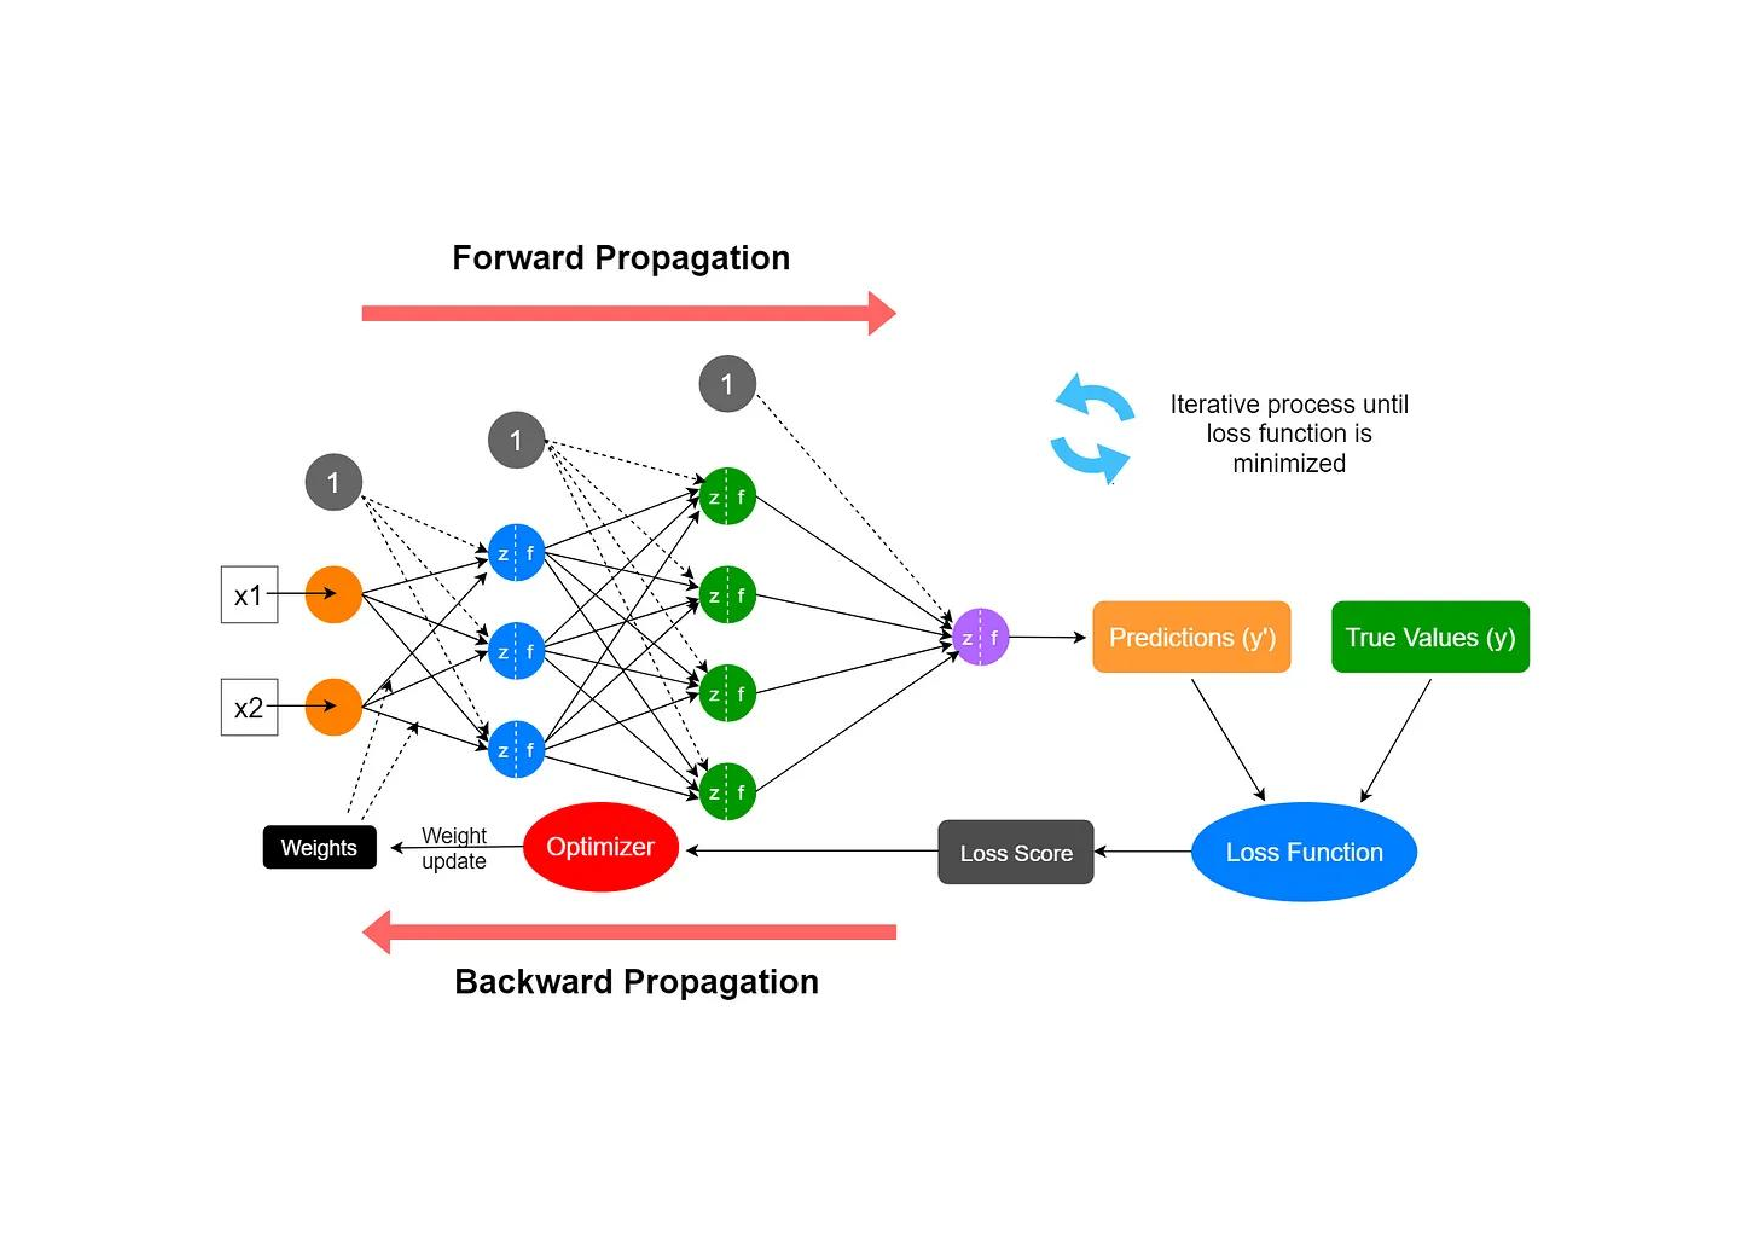
\includegraphics[width=\textwidth]{img/NeuralNetwork.pdf}\\
    \caption{ Neuronales Netz \cite{pramodithaOverviewNeuralNetwork2022a}}\label{fig:NN}
\end{figure}

  
Dabei unterscheiden sich Neural Networks in 
\gls{CNN} und \gls{RNN}.

CNNs, 
werden in der Erkennung von visuellen Daten eingesetzt, 
da sie Muster erkennen und so Objekte eindeutig identifizieren können.
Dabei werden neue Schichten wie die Konvolutionale Schicht, Pooling-Schicht und
die vollständig verbundene (FC(fully connected)) Schicht eingeführt. 
\cite{WasSindKonvolutionale2021}

Bei RNNs werden Sequenzen in die Eingabeschicht übergeben, 
wie z.B. Sätze, 
in dem jedes Wort von dem davor und dahinter abhängig ist. 
Dies ist vorallem bei der Identifizierung von natürlicher Sprache 
und umgangssprachlichen Redewendungen nützlich und  
Standardfloskeln identifizieren und nutzen zu können.
\cite{WasSindRekurrente2023}
Heutige KI-Modelle basieren auf diesen Techniken plus einigen Verbesserungen,
wie \gls{LSTM}, \gls{GRU} 
oder echo state network (ESN).
\\
\\
\paragraph{KI-Modell}
Ein KI-Modell ist das neuronale Netz mit seinen Gewichtungen. 
Vortrainierte Modelle sind z.B. GPT-3 (Generative Pre-trained Transformer Version 3).
\cite{KuenstlicheIntelligenzKI}
Durch die Eingabe eines Inputs (bei Chat-GPT zumeist Text oder Bild) 
wird ein Output in Bezug auf den Input durch das Modell erzeugt.
\\
\\
\paragraph{}
Dabei ist wichtig festzuhalten, dass bestehende KIs keine 
eigene Intelligenz besitzen, sondern diese nur Simulieren 
und auf Input angewiesen sind. Außerdem sind sie für 
verschiedene Aufgaben spezialisiert und somit als Werkzeug zu sehen. 
Die Entwicklung einer starken KI stellt eine Erschaffung von Intelligenz dar,
welche eigenständig ist und ohne Input Erfindungen erzeugt.

\subsubsection{Genetic Breeding}
Ein weiterer kleiner Teil von generativen KIs ist das Genetic Breeding, 
hier werden evolutionäre Algorithmen genutzt, 
um durch Mutation, Selektion und Rekombination 
neue Algorithmen oder Lösungen zu generieren, 
ähnlich wie in der Natur bei der Evolution von Organismen.
Dieser Prozess ermöglicht es, Lösungen zu entwickeln, 
die nicht explizit von Menschen programmiert wurden, 
sondern sich durch die "Zucht" von Algorithmen 
selbst entwickeln.
Erfindungen die aus Genetic Breeding enstehen werden derzeit
oft als zu generisch und zufällig betrachtet, 
um die Anforderungen an ein Patent zu erfüllen und bieten
derzeit noch zu wenig technische Spezifikationen 
um eine Patentierung zu gewährleisten 
\cite{hartmannKuenstlicheIntelligenzIm2020}.




\newpage


    \chapter{Patentierbarkeit von KI generierten Erfindungen und Computerprogrammen \label{cha:chapter3}}


\section{Einführung in das Patentrecht\label{sec:Patentrecht}}


Das \gls{DPMA} ist die zentrale Behörde in Deutschland, 
die für den Schutz von geistigem Eigentum zuständig ist und 
beschreibt den Nutzen von Patenten wie folgt:
\\
\\
\textit{''Mit Patenten können Sie Ihre technischen Erfindungen 
(innovative Produkte oder Verfahren) vor unerwünschter Nachahmung schützen. 
Patente belohnen ihren Inhaber 
oder ihre Inhaberin durch ein befristetes und räumlich begrenztes Nutzungsmonopol.''} 
\cite{DPMAPatentschutz}
\\
\\
Das Bundespatentgericht (BPatG) ist für Streitigkeiten über Patente zuständig, 
insbesondere für Nichtigkeitsklagen und Beschwerden gegen Entscheidungen des DPMA.

Das deutsche Patentgesetz(PatG) \cite{PatGNichtamtlichesInhaltsverzeichnis} 
regelt die rechtlichen Rahmenbedingungen für Patente in Deutschland.
Das Patentrecht in Deutschland ist ein spezieller Teil des gewerblichen Rechtsschutzes, 
der wiederum zum Bereich des Immaterialgüterrechts gehört. 
Es ist durch das Grundgesetz geschützt, insbesondere durch Art. 14 GG, 
der das Eigentum und das Erbrecht gewährleistet. 
Im materiellen Sinne gehören Patente zum Eigentum.
Ein weiterer Teil des Immaterialgüterrechts ist das Urheberrecht. 
Dieses grenzt sich von anderen Teilen des
gewerblichen Rechtsschutzes wie das Markenrecht und Designrecht dadurch ab, das 
es kreative Leistungen schützt\cite{GewerblicherRechtschutzUnd}. 


Ein Patent kann gemäß §49 Abs.1 PatG von der Prüfstelle des DPMA erteilt werden. 
Um die Patentierbarkeit von durch künstliche Intelligenz geschaffener Computerprogramme 
zu prüfen fokussiert sich diese Arbeit auf die Erteilung von Patenten. 
Die Erteilung von Patenten lässt sich in formelle und materielle Vorrraussetzungen 
gliedern, was sich aus §49 Abs.1 PatG ableitet. 
Das Deutsche Patent- und Markenamt prüft auf Antrag (§44 Abs.1 PatG) 
die formellen und materiellen Vorrausetzungen.

\section{Formelle Vorraussetzungen}

Zu den formellen Vorraussetzungen gehören:
\begin{enumerate}
    \item Anmeldung und Form, §§ 34, 37 und 38 PatG 
    \vspace{-0.11in} 
    \item Beseitigung gerügter Mängel, § 45 Abs. 1 PatG
\end{enumerate}

Patente müssen angemeldet werden (§ 34 Abs. 1 PatG). 
Gemäß § 34 Abs. 3 PatG muss die Anmeldung den Namen der/des Anmelders*in 
(Nr. 1), einen Antrag auf Erteilung des Patents, 
in dem die Erfindung kurz und genau bezeichnet ist (Nr. 2), 
einen oder mehrere Patentansprüche (Nr. 3), 
eine Beschreibung der Erfindung (Nr. 4) sowie die Zeichnungen, 
auf die sich die Patentansprüche oder die Beschreibung beziehen (Nr. 5), 
enthalten. 
Außerdem muss die Erfindung vollständig und deutlich offenbart sein (§ 34 Abs. 4 PatG) 
und nur eine einzige Erfindung enthalten (§ 34 Abs. 5 PatG). 
Paragraph 37 des PatG befasst sich mit der korrekten Erfinderbennenung 
und Paragraph 38 mit Änderungen der Anmeldung. 
\\

Sind die oben genannten formellen Anforderungen nicht erfüllt § 45 Abs. 1 PatG, 
wird der Anmelder aufgefordert, diese innerhalb einer bestimmten Frist zu beseitigen.

Wenn die gerügten Mängel beseitigt wurden 
oder es gemäß §§ 34, 37 und 38 PatG keine gerügten Mängel gibt 
sind die formellen Vorrausetzungen für die Erteilung eines Patents erfüllt.

Bei der Patentierbarkeit von KI generierten Erfindungen ist ein besonderes Augenmerk
auf § 34 Abs. 3 PatG Nr.1 zu werfen, da hier keine natürliche Person
die Erfindung hergestellt hat sondern eine KI.

\subsection{KI als Erfinder}
Die Bennung der KI als Erfinder ist ziemlich naheliegend, 
da in § 124 PatG zur Vollständigigkeit und Wahrheit vor dem
Deutschen Patent- und Markenamt, 
dem Patentgericht und dem Bundesgerichtshof aufgerufen wird.
\\
Am 17.10.2018 ging beim \gls{EPA} ein Patent ein, 
welches eine leere Zeile als Erfinder aufwies und später mit 
dem Namen der KI 
"DABUS"(Device for the Autonomous Bootstrapping of Unified Sentience) 
als Erfinder ergänzt wurde. 
Das EPA hat daraufhin entschieden, 
dass diese Bennenung nicht dem Artikel 81 Abs.19 (1) \gls{EPÜ}  genügt,
da der Erfinder eine natürliche Person sein muss, sowie ein 
Familienname, Vorname und eine Adresse angegeben werden muss.
Damit sind die formellen Vorrausetzungen an das Patent mit dem Aktenzeichen
EP 18 275 163 nicht erfüllt und das Patent wurde nicht erteilt. 
Außerdem wurde entschieden, das Namen die Dingen gegeben werden nicht
mit Namen natürlicher Personen gleichzusetzen sind. Maschinen oder KI
Systeme haben keine Rechte, die durch den Namen ausgeübt werden können 
\cite{EPA27012020}. 
In einem Beschluss vom 20.Oktober 2020 wird das Thema im Europäischem
Parlament nochmals aufgegriffen und erkannt, 
dass die aktuelle Gesetzeslage nur Erfindungen berücksichtigt,
die von Menschen mit Hilfe von KI geschaffenen wurden. 
Eine klare Unterscheidung muss getroffen werden um diese 
von vollständig autonom von KI geschaffenen Erfindungen abzugrenzen
\cite{TextsAdoptedIntellectual}.
Eine Studie, welche von der EU Kommission beauftragt wurde 
sieht die derzeitige Gesetzeslage dahingegen als ausreichend 
und fordert erst Handlungsbedarf bei dem Einsatz von starken KIs.
Es wird vorgeschlagen dann ein spezifisches Roboterrecht zu schaffen, 
um den Umgang mit intelligenten Maschinen zu regeln 
und die Informationssicherheit zu gewährleisten
\cite{gutaAPPLICABILITYGDPRARTIFICIAL2022}.
Jedoch ist es auch heute schon möglich teilweise 
Unabhängigkeit von menschlicher Einwirkung
zu schaffen, da auch schwache KIs durch Deep Learning 
Fähigkeiten nach einwirken durch den Menschen erlangen, wie bei DABUS
\cite{surdenMachineLearningLaw}\cite{dornisDornisSchopfungOhne2021}.
Eine weitere Form autonomer KIs sind die Genetic Breeding Algorithmen,
welche auch einen minimalen menschlichen Input beim Erschaffungsprozess 
verlangen.
\\
Bei der Anmeldung vor dem DPMA am 17. Oktober 2019 mit dem Aktenzeichen
10 2019 129 136 kann die künstliche Intelligenz 
DABUS ebenfalls nicht als Erfinder in Kraft treten. 
Eine künstlichen Intelligenz, 
erfüllt nicht die gesetzlichen Anforderungen an die Erfinderbenennung 
gemäß § 37 PatG und § 7 PatV. In § 7 PatV wird ebenfalls
Familienname, Vorname und eine Adresse gefordert. 
Die KI "DABUS" wird vom DPMA ebenfalls als 
Sache bzw. Machine angesehen, welche kein Träger von Rechten sein kann.
Wenn der Anmelder der einzige ist, 
der die Maschine genutzt hat, 
und keine andere Person zur Erfindung beigetragen hat, 
kann er sich selbst als Erfinder benennen. 
Falls der Anmelder Bedenken hat, 
die Nutzung der künstlichen Intelligenz zu verschweigen, 
kann er die Nutzung in der Beschreibung der Patentanmeldung angeben 
und so der Wahrheitspflicht gemäß § 124 PatG gerecht werden.
\cite{BPatG21122021}.
Einen weiteren Ansatz schlagen Konertz und Schönhof mit einem 
„erfinderloses Patent“ vor, das es der Person, 
die das Computersystem nutzt, erlaubt, 
die Rechte an der durch die Maschine generierten Erfindung zu beanspruchen
\cite{konertzErfindungenDurchComputer2018}.

\subsection{De lege lata}
Nach geltendem Recht "de lege lata" ist es in Deutschland und Europa
derzeit nicht möglich eine KI als Erfinder in Erscheinung treten zu lassen.
Die Gesetzeslage sieht vor, dass ein Erfinder eine natürliche Person sein muss
dabei ist es egal, ob eine "schwache KI" oder eine "starke KI" verwendet wurde.
Als Erfinder tritt dann der Nutzer der KI ein, welcher diese dann offiziell
als Werkzeug benutzt hat um eine technische Erfindung zu produzieren.

\subsection{De lege ferenda}
Nach zukünfigem Recht könnte sich einiges tun, die Debatte wird von verschiedenen 
Instanzen wie dem europäischen Parlament immer wieder aufgenommen und es 
werden in Zukunft weitere Fälle von Erfindungen folgen die eine klare rechtliche 
Klärung bedürfen. 
Bei den bisherigen schwachen KIs ist es noch möglich die KI als Werkzeug
zu sehen, wobei es dort schon Schwierigkeiten geben könnte, wenn eine KI,
welche durch einen Genetic Breeding Algorithmus erstellt würde eine Erfindung
schafft, ohne vorher einen Input bekommen zu haben.
Ab dem Punkt, wo kein Mensch mehr im Erfindungsprozess beteiligt,
sondern nur beim Entwicklungsprozess der KI beteiligt ist,
braucht es auf jeden Fall ein zusätzliches Recht, wie das 
oben erwähnte spezifische Roboterrecht.
Starken KIs werden spätestens, eine klare rechtliche Abgrenzung 
brauchen, 
da ab diesem Punkt Erfindungen komplett autonom von einer KI erschfaffen werden.
Dann stellt sich die Frage ob die KI doch als Erfinder auftreten kann 
und eigene Rechte besitzen darf. Ähnlich wie in dem Entwurf des Europäischen
Parlaments vom 31.5.2016 mit Empfehlungen an die Kommission zu zivilrechtlichen Regelungen im
Bereich Robotik \cite{delvauxMitEmpfehlungenKommission}. Dieser schlägt 
eine Einführung eines eigenen Rechtsstatus 
für Roboter als "elektronische Personen" vor die Rechte und Pflichten zu haben, 
ähnlich wie Menschen.
\\
\subsection{Exkurs: Internationales Patentrecht\label{sec:intp}}
\todo{exkurs1}
\section{Materielle Vorrausetzungen}

Die materiellen Vorraussetungen der Patentanmeldung sind 
in den Paragraphen §§ 1 – 5 PatG geregelt 
und lassen sich unterteilen in folgende Punkte:

\begin{enumerate}
    \item Erfindung auf einem Gebiet der Technik, § 1 Abs. 1 PatG
    \begin{enumerate}
    \vspace{-0.05in}
    \item Ausschluss, §§ Art. 1 Abs. 3 PatG und § 1 Abs. 4 PatG
    \end{enumerate}
    \vspace{-0.11in} 
    \item Neuheit, § 1 Abs. 1 i.V.m. § 3 PatG
    \vspace{-0.11in} 
    \item Erfinderische Tätigkeit, § 1 Abs. 1 i.V.m. § 4 PatG
    \vspace{-0.11in} 
    \item Gewerbliche Anwendbarkeit, § 1 Abs. 1 i.V.m. § 5 PatG
    \vspace{-0.11in} 
    \item Ausschluss, § 2 PatG
\end{enumerate}

\subsection{Technische Erfindung}

Im ersten Absatz des ersten Paragraphen im Patentgesetz wird festgelegt,
dass eine Erfindung auf einem Gebiet der Technik liegen muss, neu sein und
gewerblich anwendbar.
Eine technische Erfindung liegt laut Haedicke dann vor, 
wenn die Erfindung aus dem Bereich der Physik, 
Chemie oder den Ingenieurswissenschaften ist, 
welche sog. Gebiete der Technik darstellen.
In den letzen Jahrzehnten hat sich der Begriff 
"Technik" auch auf Erfindundungen der Biotechnologie, 
Telekommunikations- und Computertechnologie ausgeweitet 
\cite{haedickeEinfuhrung2020}
Der \gls{BGH} erstellte die
sog. „Rote-Taube“-Formel, welche technisch als  
„eine Lehre zum planmäßigen Handeln 
unter Einsatz beherrschbarer Naturkräfte zur Erreichung eines 
kausal übersehbaren Erfolgs definiert.“\cite{BGH27031969}  
Dabei genügt es „wenn die beanspruchte Lehre den Einsatz technischer Geräte umfasst“
\cite{BGH3020152015}\cite{BGH2420112011a}. 
Aufgrund der ständigen Entwicklung lässt sich 
jedoch der Begriff der „technischen Erfindung“ 
nicht abschließend definieren \cite{haedickeEinfuhrung2020}.
\\
In Paragraph 1 Abs. 3 PatG werden Gegenstände und Tätigkeiten festgelegt, 
die nicht als Erfindung angesehen werden dürfen. 
Diese sind nicht patentfähig als solche (§ 1 Abs. 4 PatG). 
Ausgeschlossene Erfindungen sind Entdeckungen, 
sowie wissenschaftliche Theorien und mathematische Methoden, 
ästhetische Formschöpfungen, Pläne, Regeln und Verfahren für gedankliche Tätigkeiten, 
für Spiele 
oder für geschäftliche Tätigkeiten sowie Programme für Datenverarbeitungsanlagen, 
sowie die Wiedergabe von Informationen (§. 1 Abs. 3 PatG). 
\\

\subsubsection{Patentierbarkeit von Computerprogrammen}
Der Punkt Programme für Datenverarbeitungsanlagen sind grundsätzlich
von der Patentierbarkeit ausgeschlossen stellt Schwierigkeiten in der 
Patentierbarkeit von durch künstliche
Intelligenz geschaffener Computerprogramme dar. 
Jedoch betrifft der Ausschluss nur Programme "als solche", 
was bedeutet, 
dass Computerprogramme in bestimmten Zusammenhängen patentierbar sind, 
wenn sie eine technische Aufgabe lösen und technische Merkmale aufweisen.
Beispiele für patentierbare Software sind technische Anwendungsprogramme, 
die Messergebnisse verarbeiten, 
technische Einrichtungen überwachen oder in technische Systeme eingreifen
\cite{RedekerITRechtSchutz}.
Bevor Beispiele von patentierbaren Computerprogrammen folgen, ist es
nötig den Begriff des Computerprogrammes eindeutig zu definieren.
Ein Computerprogrammm ist laut ISO/IEC 2382-1:1993 
eine Kombination von Anweisungen und Deklarationen in einer
Programmiersprache, die einen Computer dazu bringen, 
Funktionen zur Lösung eines Problems auszuführen 
\cite{instituteofelectricalandelectronicsengineersinc.ISO47652010}.
Das in der Programmiersprache geschriebene Programm(Quellprogramm) wird 
mittels eines Sprachcompilers in ein in Maschinensprache geschriebenes 
Programm(Objektprogramm) aus Nullen und Einsen umgewandelt \cite{WasIstProgramm}.
Computerprogramme werden nach dem Wirtschaftslexikon Gabler in Systemprogramme
und Anwendungsprogramme unterteilt. 
Ein Anwendungsprogramm löst dabei eine bestimmte Aufgabe des Anwenders, 
wie z.B. Ticketreservierungen oder Parkraumüberwachung 
\cite{lackesDefinitionAnwendungsprogramm}. 
Während ein Systemprogramm ein Bestandteil des Betriebssystems ist und 
für den Nutzer nicht sichtbare Teile der internen Steuerung des Computer übernimmt,
wie die Orchestrierung der als nächstes zu bearbeitenden Aufgabe \cite{lackesDefinitionSystemprogramm}.
Für beide Arten von Programmen gibt es mögliche Ausprägungen, 
welche patentierbar sein können, so kann ein mögliches Szenario bei einem Anwendungsprogramm sein,
dass ein Algorithmus entwickelt wurde der in der Branche noch nicht vorhanden ist. Z.B. ein
Bildverarbeitungsprogramm, das einen neuen Algorithmus verwendet, um Bilder zu verbessern.
Oder im Falle von Systemprogrammen ein Betriebssystem mit einem 
innovativen Verfahren zur Erkennung und Verhinderung von Malware.
\paragraph{Abgrenzung zur Software}
Ein Begriff der heutzutage oft synonym zu dem Begriff Computerprogramm benutzt wird,
ist Software. Software ist laut ISO/IEC 2382-1:1993 eine Sammlung von Computerprogrammen, 
Daten und Bibliotheken und somit ist ein Computerprogramm nur ein Bestandteil einer Software.
Software verwendet Computerprogramme als Tools um individuelle Anweisungen auszuführen 
\cite{ComputerProgrammeUnverzichtbareComputerprogramme}.
Software wird nach dem oben genannten ISO-Standard außerdem in 
Systemsoftware, Unterstützungssoftware und Anwendungssoftware unterteilt.
Systemsoftware ist Software, welche die Hardware des Computers steuert, 
wie z.B. Betriebssysteme oder Gerätetreiber. Unter Unterstützungssoftware 
fällt Software, die die Entwicklung und Ausführung von Anwendungssoftware
unterstützt, wie z.B. Compiler oder Texteditoren. Anwendungssoftware ist
Software, die für die Lösung von Problemen oder die Durchführung von Aufgaben
entwickelt wurden, wie z.B. Textverarbeitungsprogramme oder Spiele
\cite{instituteofelectricalandelectronicsengineersinc.ISO47652010}.
\\
\paragraph{Urteile mit Bezug auf Patentierbarkeit von Computerprogrammen}
Es gibt viele Präzendenzfälle in den Computerprogramme patentiert worden sind.
Das Europäische Patentamt erteilt außerdem Patente auch für technische Umsetzungen.
Auch wenn eine mathematische Methode keine direkte technische Anwendung hat, 
kann sie patentierbar sein, 
wenn sie speziell für eine technische Umsetzung angepasst wurde. 
Beispiele sind Optimierungen für Hardware-Architekturen, 
wie die Nutzung von GPUs für maschinelles Lernen \cite{MathematischeMethoden}. 
Eingehend beschäftigt mit der Thematik haben sich bereits einige Juristen,
wie z.B. 
Hon. Prof. Dr. iur. Klaus-J. Melullis
(Leiter der Forschungsgruppe Patentrecht am Karlsruher Institut für Technologie) und 
Dr. Matthias Koch (Rechtsanwalt beim BGH)\cite{melullisEPUArt522023} im Zusammenhang 
mit dem Europäischen Patentübereinkommen 
oder Prof. Dr. jur. Dr. rer. pol. Jürgen Ensthaler 
(Lehrstuhlinhaber für Wirtschafts-, Unternehmens - und Technikrecht an der TU Berlin)
im Zusammenhang mit dem deutschen PatG.
\cite{ensthalerEnsthalerBegrenzungPatentierung2013}.
Als Beispiel für ein Computerprogrammpatent auf deutscher 
Ebene dient die Analyse 
und Steuerung eines Flugzeugzustands.
Das hier genutzte Computerprogramm benutzt ein Verfahren, 
das anhand von Messwerten Erkenntnisse 
über den Zustand eines Flugzeugs gewinnt und 
die Funktionsweise eines Systems beeinflusst 
\cite{BGH3020152015}.
Hier liegt eine technische Problemlösung vor, 
da die Methode zur Steuerung eines technischen Systems eingesetzt wird.
Das Europäische Patentamt hat mit dem Patent EP0005954 
„Verfahren und Vorrichtung zur verbesserten digitalen Bildverarbeitung“ 
einen entscheidenden Meilenstein gesetzt, 
der den Weg für die Patentierbarkeit mathematischer Methoden und 
Computerprogramme geebnet hat.
Das hier aufgeführte Computerprogramm ist ein 
Verfahren zur digitalen Bildverarbeitung \cite{EPThisFile}.
Der technische Charakter liegt in der Verbesserung 
der Bildqualität durch ein spezielles Filterverfahren.
\\
Die bloße Implementierung einer Rechenmethode auf einem Computer 
verleiht ihr noch keinen technischen Charakter. 
Entscheidend ist die konkrete Anwendung der Methode 
in einem technischen Zusammenhang, der einen unmittelbaren Effekt in der 
physischen Welt erzeugt \cite{melullisEPUArt522023}.
So sind mehrere Patente abgelehnt worden,
wie, Verfahrenen, 
die lediglich der Auswertung von Daten auf statistischer Basis dienen.
Dies war der Fall bei den Beschlüssen 17 W (pat) 74/07\cite{BPatG10012012}
und 17 W (pat) 6/00 \cite{BPatG01032001} vom Bundespatentgericht.
Das EPA sieht Verfahren zum Sammeln und Auswerten von Daten 
im Rahmen von betriebswirtschaftlichen Prozessen als nicht patentfähig an 
(siehe T 154/04 \cite{EuropaischesPatentamt152006}),
da sie kein technisches Problem lösen.
\\
Nach dieser Definition von Computerprogrammen und der Klärung von dem Begriff
"Technik" kann nun eine Abschätzung getroffen werden, 
ab wann Computerprogramme patentierbar sind. 
Durch die verschiedenen Urteile wird außerdem sichtbar 
ab wann ein Computerprogramm als technisch angesehen wird.
Jedoch bleibt die Patentierbarkeit von Computerprogrammen 
ein komplexes und umstrittenes Thema 
und internationale Standards könnten 
langfristig mehr Klarheit und Konsistenz schaffen.
Viele Computerprogrammpatente wurden erst abgelehnt und erst nach 
einer Beschwerde und erneuter Prüfung erteilt.
Wege um das Patentgesetz dahingehend zu vereinfachen schlägt 
Prof. Dr. jur. Dr. rer. pol. Jürgen Ensthaler vor. 
Eine mögliche Lösung wäre, die „als solche“-Formel durch eine Regelung zu ersetzen, 
wie sie für Gensequenzen in § 1a PatG besteht. 
Demnach könnten Algorithmen nur dann patentiert werden, 
wenn die konkrete technische Funktion klar benannt 
und in den Patentanspruch aufgenommen wird. 
Diese Funktionsbegrenzung würde verhindern, 
dass abstrakte mathematische Lehren, 
die für viele Anwendungen nutzbar sind, patentiert werden 
\cite{ensthalerEnsthalerBegrenzungPatentierung2013}. 
\subsection{Exkurs: Urheberrecht\label{sec:urh}}
\todo{exkurs2}






\subsection{Neuheit}
Eine Erfindung gilt als neu, wenn sie nicht zum Stand der Technik gehört. 
Der Stand der Technik umfasst alle Kenntnisse, 
die vor dem für den Zeitrang der Anmeldung
maßgeblichen Tag durch schriftliche 
oder mündliche Beschreibung, durch Benutzung oder in
sonstiger Weise der Öffentlichkeit zugänglich gemacht worden sind (§ 3 Abs. 1 PatG).
Als Stand der Technik gilt auch der Inhalt nationaler Patentanmeldungen 
in der beim Deutschen
Patentamt ursprünglich eingereichten Fassung mit älterem Zeitrang, 
die erst an oder nach dem für
den Zeitrang der jüngeren Anmeldung maßgeblichen Tag der Öffentlichkeit 
zugänglich gemacht
worden sind (§ 3 Abs. 2 Nr. 1 PatG). 
Bei KI-generierten Erfindungen kann es schwierig sein, 
den Stand der Technik umfassend zu bestimmen. 
KI-Modelle können auf umfangreiche Daten zugreifen und Lösungen generieren, 
die in kleinen Teilen bereits veröffentlicht, 
aber in dieser spezifischen Kombination noch nicht dokumentiert sind.
Im Kontext von KI stellt sich hier die Frage 
ob eine Erfindung überhaupt als neuartig angesehen werden kann, 
da KI basierte Erfindungen meist aus der Analyse großer Datenmengen bestehen
und der Generierung von Output aus diesen. 
Es werden nur bestehende Muster im Stand der Technik kombiniert 
und so nur durch Kombination aus anderen konkreten technischen Lösungen, 
welche bereits in irgendeiner Form öffentlich zugänglich waren ein neue generiert.
Eine Kombination bekannter technischer Lösungen kann als „neu“ angesehen werden,
wenn genau diese spezifische Kombination zuvor nicht offengelegt wurde, 
eine neu Ordnung von Informationen stellt jedoch keine Neuheit dar.
Dabei stellt sich jedoch die Frage ob die Kombination naheliegend und
somit keine erfinderische Höhe aufweist.

\subsection{Erfinderische Tätigkeit}
Eine Erfindung gilt als auf einer erfinderischen Tätigkeit beruhend, 
wenn sie sich für den Fachmann
nicht in naheliegender Weise aus dem Stand der Technik ergibt (§ 4 S. 1 PatG). 
Gehören zum Stand
der Technik auch Unterlagen im Sinne des § 3 Abs. 2 PatG, 
so werden diese bei der Beurteilung der
erfinderischen Tätigkeit nicht in Betracht gezogen (§ 4 S. 2 PatG).
In vielen Fällen agiert die KI als eine Art „Black Box“, 
bei der die Inputs vom Menschen bereitgestellt werden, 
die endgültigen Outputs jedoch nicht vollständig nachvollziehbar sind 
\cite{pauliniKIgenerierteErfindungPatentrechtliche}. 
Um die erfinderische Tätigkeit sinnvoll beurteilen zu können
muss klar sein, wie die KI zu ihrem Ergebnis kam. 
Wenn der Output für den Fachmann nicht aus dem bereits bekannten 
ableitbar ist, ist eigentlich eine erfinderische Tätigkeit gegeben.
Jedoch ist die erfinderische Tätigkeit so leicht zu reproduzieren,
dass eine erfinderische Höhe als fraglich angesehen werden kann.
Somit stellt sich die Frage: 

Ist nun auch dem Stand der Technik zugehörig alles was durch eine KI aus dem 
Stand der Technik hergeleitet werden kann? 

Dr. Joel Nägerl, Dr. Benedikt Neuburger und Dr. Frank Steinbach beschäftigen
sich mit dieser Thematik und kommen zu dem Schluss,
dass der Fachmann, der Beurteilungen vornimmt, 
in Zukunft KI-gestützte Systeme als „Lesebrille“ verwenden könnte.
Dies könnte dazu führen, dass Erfindungen, 
die heute noch mit einer erfinderischen Tätigkeit bewertet werden, 
in der Zukunft als naheliegend betrachtet und somit nicht patentierbar wären.
Dabei ist jedoch entscheidend, 
dass nur solche KI-Systeme herangezogen werden dürfen, 
die zum Zeitpunkt der Patentanmeldung verfügbar und gängig sind. 
Es ist unzulässig, den Bewertungsmaßstab durch die nachträgliche Nutzung 
einer später entwickelten, leistungsstärkeren KI zu erhöhen 
\cite{nagerlKunstlicheIntelligenzParadigmenwechsel2019}.

Insgesamt ist die Bewertung der erfinderischen Tätigkeit
von KI-generierten Erfindungen derzeit stark von der juristischen Auslegung abhängig. 
Solange der Beitrag der KI nicht klar und nachvollziehbar ist, 
bleibt es schwierig, 
die erfinderische Tätigkeit von KI-Erfindungen 
im patentrechtlichen Sinne zu bewerten.
Die Gesetzeslage könnte sich dem entsprend weiterentwickeln, 
die Reichweite 
vom Stand der Technik auf den Entwicklungshorizont von KI auszuweiten.
Dies ist bei dem derzeitigen Stand von KI durchaus sinnvoll,
jedoch ab der ersten starken KI vollkommen hinfällig.
\\
\subsection{Gewerbliche Anwendbarkeit}
Eine Erfindung gilt als gewerblich anwendbar, 
wenn ihr Gegenstand auf irgendeinem gewerblichen
Gebiet einschließlich der Landwirtschaft hergestellt 
oder benutzt werden kann (§ 5 PatG).
Das Erfindungen, 
welche mit/durch KI entstanden sind gewerblich anwendbar sind ist durchaus möglich.
KI-Systeme wie AlphaFold von DeepMind haben Fortschritte 
in der Medikamentenforschung ermöglicht, 
indem sie die 3D-Struktur von Proteinen präzise vorhersagen \cite{AlphaFold2024}.
\\




    \chapter{Hypothetischer Patentantrag\label{cha:chapter5}}

\section{Vorbereitung der Patentanmeldung}

Um ein Patent beim DPMA Anzumelden wird ein Anmeldeformular benötigt (Formular P 2790),
welches im Internet unter \url{https://www.dpma.de/docs/formulare/patent/p2007.pdf} heruntergeladen
werden kann. 
Eine ausschließlich Windows kompatible Alternative bietet
das DPMA direktPro-System zur Online Anmeldung von Patenten.

Das Anmeldeformular verlangt:

\begin{enumerate}
    \item Angaben zum Anmelder
    \item Erfindernennung (falls abweichend vom Anmelder)
    \item Titel der Erfindung, Art der Erfindung
    \item Prioritätsangaben (falls in mehreren Ländern eingereicht)
    \item Angaben zu den Unterlagen (beigefügte Dokumente)
    \item Wahl des Prüfungsverfahrens (inhaltliche Prüfung des Antrags)
	\item Zahlungsweise
\end{enumerate}

Dabei ist zu beachten, das die Wahl des Prüfungsverfahrens 
(Rechercheantrag (§ 43 Patentgesetz)) oder
Prüfungsantrag (§ 44 Patentgesetz) zusätzliche einmalige Kosten verursacht.
Bei Auslassen der Wahl des Prüfungsverfahrens wird eine rein formulare
Prüfung des Patentantrages durchgeführt und keine inhaltliche.
Erfolgt lediglich eine Formalprüfung wird das Patent nicht erteilt.
Weitere Bestandteile der Patentanmeldung sind laut DPMA \cite{DPMAAnmeldung}:

\begin{enumerate}
	\item Technische Beschreibung der Erfindung, gegebenenfalls mit Bezugszeichenliste
	\item Patentansprüche
	\item Zeichnungen, falls von Ihnen als notwendig erachtet
	\item Zusammenfassung
	\item Erfinderbenennung
\end{enumerate}

Diese Dokumente werden mit dem Punkt Angaben 
zu den Unterlagen (beigefügte Dokumente) abgedeckt.

\section{Erstellung KI-Patent}

Um eine durch KI entwickelte Erfindung zu generieren, 
welche relativ wenig durch den Input beeinflusst wurde, 
wird der Input:
"Erstelle eine patentierbare technische Erfindung 
in Form eines Computerprogrammes im Bereich Iot" in ChatGPT-4o eingegeben.
Die daraus entstandene Erfindung lautet:
Intelligentes Energiemanagementsystem für \gls{IoT}-basierte Haushalte.
Als Anmelder tritt wie in Kapitel 3 durch den BGH festgelegt der Benutzer
der KI in Erscheinung \ref{cha:chapter3} \ref{fig:Pat1-3}.
\begin{figure}[htb]
    \centering
    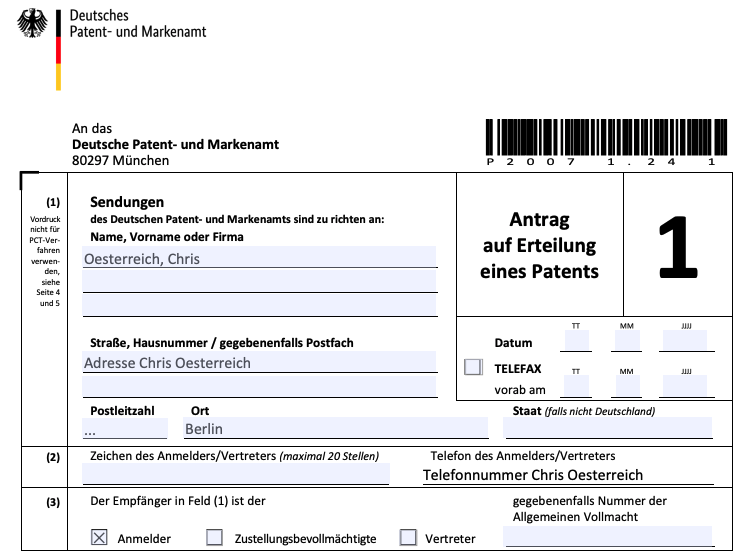
\includegraphics[width=\textwidth]{Patentanmeldung1-3.png}\\
    \caption{ Patentanmeldung Schritte 1-3 }\label{fig:Pat1-3}
\end{figure}
\\
Damit sind die Punkte "Angaben zum Anmelder" und "Erfindernennung" bearbeitet, 
da der Erfinder hier gleich dem Anmelder ist.
Die Bezeichnung der Erfindung ist:
Intelligentes Energiemanagementsystem für IoT-basierte Haushalte.
Die hypothetische Patentanmeldung soll sowohl einen Prüfungsantrag, 
als auch einen Rechercheantrag beinhalten \ref{fig:Pat6-7}.
\begin{figure}[htb]
    \centering
    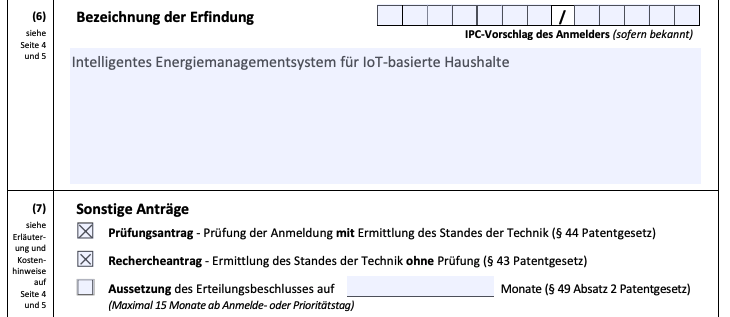
\includegraphics[width=\textwidth]{Patentanmeldung6-7.png}\\
    \caption{ Patentanmeldung Schritte 6-7 }\label{fig:Pat6-7}
\end{figure}
\\
\\
Für den Rechercheantrag fällt eine Gebühr von 300 Euro an (Stand 2024),
für den Prüfungsantrag 150 Euro, in Kombination mit dem Rechercheantrag (Stand 2024).
Bei Anmeldung in Papierform bis zu 10 Patentansprüche fällt außerdem noch eine
Anmeldegebühr von 60 Euro an (Stand 2024). Bei jedem weiteren Anspruch
fallen 30 Euro pro Anspruch an(Stand 2024) Dies ergibt für das obige Patent 
eine Anmeldegebühr von 570 Euro \ref{fig:Pat10}.
\begin{figure}[htb]
    \centering
    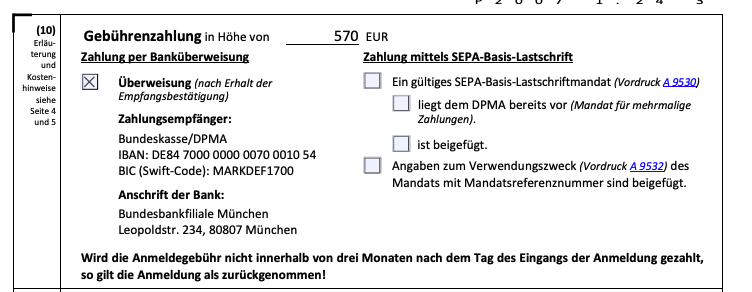
\includegraphics[width=\textwidth]{Patentanmeldung10.png}\\
    \caption{ Patentanmeldung Schritte 10 }\label{fig:Pat10}
\end{figure}

Für die oben geforderten Anlagen sind mehr Informationen von der KI
bezüglich des Patents nötig.

Als Beschreibung der Erfindung \ref{beschPDF} gibt ChatGPT-4o eine Einordnung 
in das Technische Gebiet, den Stand der Technik, die Problemlösung,
die technischen Merkmale , sowie Vorteile der Erfindung zurück.
Patentansprüche \ref{schutzPDF} 
und eine Zusammenfassung \ref{zusammenfassungPDF} müssen in zusätzlichen Prompts 
abgefragt werden. 
Damit wären die Grundbestandteile der Patentanmeldung erfüllt und nach Angabe der 
Zahlungsweise und
Einreichung der Anmeldung beim DPMA würde die Prüfung beginnen. 

\section{Die von der KI entwickelte Erfindung}


\section{Prüfung der KI Erfindung}
Die von ChatGPT-4o entstandene Erfindung nutzt machinelles lernen um eine effiziente
Energieverwaltung in Haushalten zu ermöglichen. 





    \chapter{Auswertung\label{cha:chapter6}}

\section{Darstellung der Ergebnisse}
Das Urteil der KI "DABUS" ist wegweisend für die Patentierbarkeit von
KI-Erfindungen. In Deutschland ist per BGH-Beschluss 
festgelegt, dass eine KI
zur Erstellung von Erfindungen verwendet werden darf. Sie
darf auch den größeren Anteil an der Erstellung des Patents
haben. Ein menschlicher Anteil ist allein durch die 
fehlende Anwesenheit von komplett autonom agierenden KIs gegeben.
Der Erfinder ist die menschliche Person (oder Personen),
welche mit der KI interagiert um die Erfindung zu erstellen.
Damit sind die formellen Anforderungen bei der Anmeldung
von durch KI geschaffener Computerprogramme im deutschen
Patentrecht definiert, da sich die restlichen formellen
Anforderungen nicht von denen 
ohne KI oder ohne Computerprogrammen unterscheiden.
Die materiellen Herausforderungen bei der Patentierbarkeit
von Computerprogrammen sind vor allem die Frage der Technizität.
Da eine Erfindung auf einem Gebiet der Technik liegen muss
um patentierbar zu sein, ist es wichtig zu klären, ab wann
Computerprogramme als technisch gelten.
Diese Computerprogramme werden dann nicht von der Patentierbarkeit
ausgeschlossen. Sie sind keine Computerprogramme "als solche",
sondern welche mit technischem Charakter.
Über verschiedene Rechtssprechungen vom Dispositionsprogramm, über
das Antiblockiersystem und die Entscheidung zum Tauchcomputer sowie 
vielen weiteren, ist in Deutschland eine Rechtsgrundlage geschaffen worden
um die Technizität von Computerprogrammen zu bewerten.
Das DPMA fasst die Rechtssprechungen in einen drei Schritte Plan 
zur Beurteilung des technischen 
Charakters von computerimplementierten Erfindungen zusammen.
Eine Erfindung muss auf einem Gebiet der Technik liegen,
ein technisches Problem lösen und erfinderische Tätigkeit und Neuheit 
aufweisen. Wobei nur Aspekte berücksichtigt werden,
die die Lösung des technischen Problems beeinflussen für die
erfinderische Tätigkeit und Neuheit.
Damit lässt sich die Beurteilung der Technizität
von Computerprogrammen in Deutschland durchführen.
Wenn es um die Beurteilung des Neuheit von durch KI generierten 
Erfindungen geht, ist es wichtig zu beachten, dass eine KI 
durchaus neuartige Erfindungen hervorbringen kann.
Eine KI lernt auf historischen Daten, trotzdem ist
eine neue Kombination aus bereits bekannten Technologien, 
neuartig, wenn es sie in der bisherigen Form noch nicht gab. 
Die Frage ist dann, ob diese Form dann nicht nahliegend ist.
Eine erfinderische Tätigkeit kann trotz geringem 
zutun des menschlichen Nutzers gegeben sein, wenn 
die Nutzung für die Entwicklung der Erfindung für einen Fachmann 
im Fall von Verfahrenspatenten
nicht naheliegend ist 
oder die Erfindung an sich im Fall von Erzeugnispatenten 
nicht naheliegend ist.

Im Falle des hypothetischen Patentantrages \ref{cha:chapter5}
wurde eine Erfindung generiert, welche durch die KI ChatGPT-4o
erstellt wurde.
Die Erfindung erfüllt die nötigen formellen Vorraussetungen
unter Angabe des Nutzers der KI als Erfinder. In dem Fall
wird die KI als Werkzeug deklariert.
Da die generierte Erfindung "Intelligentes Energiemanage-
mentsystem für Internet of Things (IoT)-basierte Haushalte"
Schutzansprüche für mehrere Computerprogramme beinhaltet, 
wird der technische Charakter nach den Maßstäben des DPMA geprüft.
In diesem Fall weisen die Schutzansprüche mit 
Bezug auf Computerprogramme, bzw. Verfahren,
welche ein Computerprogramm darstellen, 
einen technischen Charakter auf und
sind keine Computerprogramme "als solche".
Die Neuheit ist bei dem erstellten Patent ebenfalls gegeben,
da die konkrete Kombination, wie sie in den Schutzansprüchen
dargestellt wurde, noch nicht Stand der Technik ist.
Jedoch bleibt die Frage der Erfinderischen Höhe bei der
Erfindung bestehen.
Dadurch, dass die Schutzansprüche, welche von der KI
erstellt wurden, den Einsatz von maschinellen
Lernen im Bereich von IoT behandeln und dies
für einen Fachmnn in diesem Bereich naheliegend
ist, ist ein Verfahrenspatent dafür nicht mit einer
erfinderischen Tätigkeit verbunden.
Außerdem bieten die weiteren Ansprüche mit Bezug auf 
Erzeugnispatente ebenfalls keine
für einen Fachmann nicht naheliegenden Innovationen,
weshalb die erfinderische Höhe bei allen Schutzansprüchen fehlt.
In Sachen erfinderische Tätigkeit 
fehlt es ChatGPT-4o an der nötigen Kreativität bei 
der von im hypothetischen Patentantrag generierten Erfindung.
Einzig und Alleine der Einsatz von ChatGPT zum Erstellen
von patentierbaren Erfindungen könnte im Bereich Iot 
als erfinderisch gelten, wird hier aber nicht als Anspruch
formuliert und geprüft.
Das hypothetische Patent ist trotz der im Prompt 
verwendeteten Anforderung von Patentierbarkeit,
nicht patentierbar. 
\section{Analyse}

Die Patentierbarkeit von durch KI 
geschaffener Computerprogramme ist ein sehr aktuelles Thema 
und es ist durchaus möglich, dass eine KI mit simplen
Inputs ein patentierbares Computerprogramm erzeugen kann.
Die formellen Vorrausetzungen der Patentanmeldung, 
dass ein Nutzer der KI als
Erinder eintritt, stellen in Deutschland keine große Hürde
dar, da die Wahrheitspflicht laut BGH hierbei
nicht verletzt wird. Die Technizität eines von einer
KI erstellten Programmes 
kann gewährleistet werden, 
indem der KI mitgegeben wird, dass das 
Computerprogramm ein technisches Problem lösen 
soll oder generell, dass es patentierbar sein soll.
Es gibt mittlerweile dutzende Fälle in denen 
Computerprogramme mit technischen Charakter patentiert wurden
und auch die oben aufgeführten Programme lösen
ein technisches Problem mit technischen Mittel und
sind durchaus patentierbar. Bei den materiellen
Vorrausetzungen der Patentanmeldung ist es Einzelfall
abhängig, ob die Erfindung genug erfinderische Tätigkeit
und Neuheit aufweist. In dem hypothetischen
Patentantrag wurde gezeigt, dass die Erfindung
schnell am Punkt der erfinderischen Tätigkeit scheitern
kann, da eine KI auf den ersten Blick kreativ erescheinde
Erfindungen liefert, diese jedoch für einen Fachmann
als sehr naheliegend angesehen werden können.
Dies kann umgangen werden indem ein Ingenieur der 
Branche indem die KI eine Erfindung generiert die 
Erfindung prüft, gegebenenfalls anpasst oder bei
mehreren die naheliegenden aussortiert. Dabei ist 
dann jedoch auch schon ein höherer menschlicher 
Aufwand mit verbunden und es stellt sich die Frage,
ob die Erfindung noch als KI generiert angesehen werden
kann, wenn es sich im ein Zusammenspiel von Mensch
und Erfindung handelt. Es ist dem BGH zuzustimmen, 
dass derzeit noch keine KI alleine etwas erfinden kann,
ohne den Input eines Menschen und es stellt sich
auch die Frage, ob eine KI ohne einen Ingenieur
oder fachkundigen in der Branche eine patentierbare
Erfindung erschaffen kann.
\section{Interpretation}
Die Analyse der Gesetzgebung und des hypothetischen Patentantrages
haben gezeigt, dass Erfindungen von KI durchaus das Potential
haben, in nächster Zeit patentierbare Computerprogramme zu
generieren. Vorallem der hypothetische Patentantrag hat gezeigt,
wie einfach es ist eine Erfindung mit einer KI, in diesem Fall
ein LLM zu generieren. Wenn eine spezialisiertere KI verwendet 
wird und diese von einem Fachmann bedient wird ist es
möglich mit wenig Aufwand viele patentierbare Erfindungen zu 
generieren. Diese werden so lange patentierbar bleiben,
bis es als naheliegend angesehen wird die verwendete KI
als Werkzeug in der Branche zu verwenden oder sich
die Rechtssprechung ändert. Die Entwicklung im 
Bereich von KI ist sehr schnell, so dass es durchaus vorstellbar
ist, dass eine Art Erfinder-KI entwickelt wird, die schaut,
wie der aktuelle Stand der Technik ist und wie sie etwas nicht 
naheliegendes erfinden kann. Die Erfindungen wären 
dann auf Relevanz und gewerbliche Anwendbarkeit zu prüfen, 
von einem Menschen oder ebenfalls von einer darauf 
trainierten KI. 
    \chapter{Fazit und Ausblick\label{cha:chapter7}}

\section{Zusammenfassung\label{sec:summary}}

Die Arbeit zeigt, 
dass die fortlaufende Entwicklung von KI neue Herausforderungen 
für das bestehende Patentrecht mit sich bringt, 
insbesondere im Hinblick auf die Patentierbarkeit 
von durch KI generierten Computerprogrammen. 
KI kann mittlerweile Aufgaben übernehmen, die 
traditionell den Einsatz menschlicher Kreativität
und Intelligenz erfordert haben. Das stellt das 
Patentrecht vor Schwierigkeiten bei 
der Fragestellung des Erfinders in Fällen,
wo KI zur Erfindungsgenerierung eingesetzt
wird oder den größten Anteil übernimmt.
Nach der aktuellen Rechtslage 
in Deutschland und Europa dürfen 
nur natürliche Personen als Erfinder benannt werden. 
Der Nutzer der KI gilt als der Erfinder, 
da die KI bislang nur als Werkzeug betrachtet wird, 
das durch einen Menschen bedient wird.
Diskussionen, 
inwieweit KI tatsächlich als Erfinder auftreten könnte,
nehmen zu. 
Das Beispiel von DABUS zeigt das KI durchaus viele
Anforderungen an die Patentierbarkeit erfüllen
kann.

Die Arbeit hat ebenfalls deutlich gemacht, 
dass das deutsche Patentrecht bereits Möglichkeiten hat, 
Patente für Computerprogramme zu erteilen, 
insofern diese eine technische Problemlösung darstellen. 
Die sog. "als solche" Regelung, welche Computerprogramme
von der Patentierbarkeit ausschließt,
gilt nicht wenn ein Computerprogramm eine technische Wirkung 
aufweist.
Damit besteht die Möglichkeit, 
Computerprogramme, die durch KI erstellt wurden, 
zu patentieren, solange sie eine technische Wirkung aufweisen 
und die formellen Voraussetzungen,
wie der Angabe des Nutzer als Erfinder, erfüllen.
Dies ist besonders spannend, da KI Computerprogramme
in den technischen Bereichen, wie 
der Automatisierung, der Bildverarbeitung oder dem Energiemanagement
erzeugen kann.
\section{Problems Encountered\label{sec:problems}}

Die größte Herausforderung bei dieser Arbeit stellt
die Aktualität dieses Themas dar und die 
schnelle Weiterentwicklung von KI-Systemen.
Die Rechtssprechung kann nicht immer mit der 
technologischen Entwicklung im Bereich KI
Schritt halten und es ist schwer
klare Rechtssprechungen zu finden. Der Fall
"DABUS" ist auch noch nicht vollständig durch das Patentverfahren
gegangen, nur die Erfinderfrage ist jetzt
geklärt. Aufgrund der Aktualität des Themas gibt
es generell wenig Rechtssprechungen, die sich auf
KI-Systeme beziehen. Im Gegensatz zu den Rechtssprechungen
zu Computerprogrammen, die schon seit den 80er Jahren
bestehen, aber auch einen gewissen Spielraum lassen,
in der Definition der Technizität eines Programmes. KI-Systeme
entwickeln sich ständig weiter und während dieser Arbeit 
ist ChatGPT von der Version 3 auf die Version 4o und mittlerweile
o1 gewechselt. Es könnte sein, dass der hypothetische
Patentantrag, welcher von einer Version o1 entwickelt 
worden wäre, nicht mehr als für
einen Fachmann naheliegend betrachtet wird. Diese Arbeit
kann einen guten Überblick über die aktuelle Rechtslage 
und für schwache KIs eine Übersicht der Patentierbarkeit geben.
Jedoch werden Anpassungen der Gesetzeslage schnell 
folgen müssen um mit der Geschwindigkeit des Fortschritts von
KIs mitzuhalten und jetzt noch gängige Praxis ist in 
einigen Jahren vielleicht schon überholt.

\section{Ausblick\label{sec:outlook}}

Die derzeitige rechtliche Lage wird durch die 
stetige Weiterentwicklung von KI-Systemen in Frage
gestellt. Das fortwährende Verschwimmen der 
Grenze zwischen menschlicher und maschineller Kreativität
dazu, dass die Anforderungen an die Bewertung von 
erfinderischer Tätigkeit und Neuheit neu definiert
werden müssen. 
Zukünftige Entwicklungen in der Patentrechtspraxis werden zeigen, 
wie weit die Automatisierung und Eigenständigkeit von KIs voranschreiten muss, 
um als juristische Person anerkannt zu werden. 
Die Arbeit zeigt auf, dass klare Regelungen notwendig sind, 
um auch in Zukunft Innovationen zu schützen 
und dabei das Gleichgewicht zwischen 
menschlicher Erfindung und KI-Unterstützung zu wahren.
Es wird aufgrund noch größerer Datenmengen die einer 
KI zur Verfügung stehen und noch kmplexeren Algorithmen
noch schwieriger den kreativen Prozess einer KI 
nachzuvollziehen. Erfindungen werden entstehen, welche
auch für einen Fachmann nicht naheliegend sind, jedoch 
technisch sehr naheliegend durch den Einsatz von KI.
Dann wird es nötig sein, dass auch der Fachmann zu einer
KI greift, um den aktuellen Stand der Technik identifizieren
zu können. 

Starke KI wird zwangsläufig irgendwann dazu 
führen, dass weitreichende Änderungen in der 
Gesetzgebung vorgenommen werden müssen. Dabei steht 
vorallem die Frage im Vordergrund, ab wann eine 
KI als eigenständige Rechtsperson angesehen werden
kann. Spätestens ab diesem Zeitpunkt ändert sich 
das gesamte Patentsystem und es werden weitere 
Maßnahmen wie die Einführung eines Roboterrechts oder
andere spezifische Gesetzgebungen für KI folgen. 
Auch eine Einführung einer sog. "elektronischen
Person" könnte in Betracht gezogen werden, um
Rechte für KI Systeme zu schaffen.
Starke KI braucht einen gesonderten Platz um 
Patentrecht, um als unabhängige Akteure 
im Innovationsprozess aufzutreten.
Es muss eine Balance zwischen dem Schutz menschlicher Kreativität 
und der Förderung von technologischer Innovation geschaffen werden
um sowohl die Vorteile von KI voll auszuschöpfen, als 
auch Fairness den gegenüber menschlichen Erindern zu 
gewährleisten.

Diese Punkte machen deutlich, 
dass der rechtliche Umgang mit KI und deren Rolle 
im Innovationsprozess einer fortlaufenden Anpassung bedarf, 
um sowohl technologische 
als auch juristische und gesellschaftlichen
Anforderungen gerecht zu werden.

    \chapter{Fazit und Ausblick\label{cha:chapter7}}
The final chapter summarizes the thesis. The first subsection outlines the main ideas behind Component X and recapitulates the work steps. Issues that remained unsolved are then described. Finally the potential of the proposed solution and future work is surveyed in an outlook.

\textbf{Approx 2 days}
\section{Zusammenfassung\label{sec:summary}}

Explain what you did during the last 6 month on 1 or 2 pages!
\\
\\
\noindent The work done can be summarized into the following work steps

\begin{itemize}
		\item Analysis of available technologies
		\vspace{-0.11in} 
		\item Selection of 3 relevant services for implementation
		\vspace{-0.11in} 
		\item Design and implementation of X on Windows
		\vspace{-0.11in} 
		\item Design and implementation of X on mobile devices
		\vspace{-0.11in} 
		\item Documentation based on X
		\vspace{-0.11in} 
		\item Evaluation of the proposed solution
\end{itemize}

\section{Problems Encountered\label{sec:problems}}

Summarize the main problems. How did you solve them? Why didn't you solve them?

\section{Ausblick\label{sec:outlook}}

Future work will enhance Component X with new services and features that can be used ...

% ---------------------------------------------------------------
\backmatter % no page numbering from here
    \newacronym{KI}{KI}{Künstliche Intelligenz}
\newacronym{DPMA}{DPMA}{Deutsches Patent- und Markenamt}
\newacronym{PatG}{PatG}{Patentgesetz}
\newacronym{BGH}{BGH}{Bundesgerichtshof}
\newacronym{EPA}{EPA}{Europäisches Patentamt}
\newacronym{EPÜ}{EPÜ}{Europäisches Patentübereinkommen}
\newacronym{IoT}{IoT}{Internet of Things}
\newacronym{CNN}{CNN}{Convolutional Neural Network}
\newacronym{RNN}{RNN}{Recurrent Neural Network}
\newacronym{LSTM}{LSTM}{Long Short-Term Memory}
\newacronym{GRU}{GRU}{Gated Recurrent Units}

    \bibliographystyle{geralpha}
    \bibliography{./bib/manual}
    
    % \addchap{Annex}

\begin{appendix}

\lstset{language=,caption=Sourcecode Listing,captionpos=b,
label=yahoowidgetkon,showstringspaces=false,
basicstyle={\fontfamily{pcr}\selectfont\footnotesize}}
\begin{lstlisting}
<?xml version="1.0" encoding="UTF-8"?>
<widget>
	 <debug>off</debug>
	 <window name="myWindow" title="Hello Widget" visible="true">
		 <height>120</height>
		 <width>320</width>
		 <image src="Resources/orangebg.png">
			<name>orangebg</name>
			<hOffset>0</hOffset>
			<vOffset>0</vOffset>
		</image>
		 <text>
			 <name>myText</name>
			 <data>Hello Widget</data>
			 <color>#000000</color>
			 <size>20</size>
			 <vOffset>50</vOffset>
			 <hOffset>120</hOffset>
		 </text>
	</window>
</widget>
\end{lstlisting}

\newpage


\lstset{caption=SIP request and response packet\cite{SIPBook},
captionpos=b,label=sippacket,showstringspaces=false,
basicstyle={\fontfamily{pcr}\selectfont\footnotesize}}
\begin{lstlisting}
INVITE sip:bob@network.org SIP/2.0
Via: SIP/2.0/UDP 100.101.102.103:5060;branch=z9hG4bKmp17a
Max-Forwards: 70
To: Bob <sip:bob@network.org>
From: Alice <sip:alice@ims-network.org>;tag=42
Call-ID: 10@100.101.102.103
CSeq: 1 INVITE
Subject: How are you?
Contact: <sip:xyz@network.org>
Content-Type: application/sdp
Content-Length: 159
v=0
o=alice 2890844526 2890844526 IN IP4 100.101.102.103
s=Phone Call
t=0 0
c=IN IP4 100.101.102.103
m=audio 49170 RTP/AVP 0
a=rtpmap:0 PCMU/8000

SIP/2.0 200 OK
Via: SIP/2.0/UDP proxy.network.org:5060;branch=z9hG4bK83842.1
;received=100.101.102.105
Via: SIP/2.0/UDP 100.101.102.103:5060;branch=z9hG4bKmp17a
To: Bob <sip:bob@network.org>;tag=314159
From: Alice <sip:alice@network.org>;tag=42
Call-ID: 10@100.101.102.103
CSeq: 1 INVITE
Contact: <sip:foo@network.org>
Content-Type: application/sdp
Content-Length: 159
v=0
o=bob 2890844526 2890844526 IN IP4 200.201.202.203
s=Phone Call
c=IN IP4 200.201.202.203
t=0 0
m=audio 49172 RTP/AVP 0
a=rtpmap:0 PCMU/8000
\end{lstlisting}


\end{appendix}

\endinput


\end{document}
